\begin{problem}
  {Q3(b)}
  ~\\
  \begin{center}
    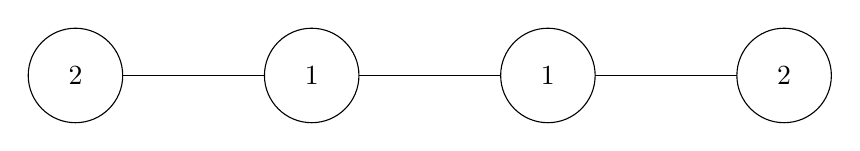
\begin{tikzpicture}[scale=0.2]
      \tikzstyle{every node}+=[inner sep=0pt]
      \draw [black] (5,0) circle (3);
      \draw (5,0) node {$2$};
      \draw [black] (20,0) circle (3);
      \draw (20,0) node {$1$};
      \draw [black] (35,0) circle (3);
      \draw (35,0) node {$1$};
      \draw [black] (50,0) circle (3);
      \draw (50,0) node {$2$};
      \draw [black] (8,0) -- (17,0);
      \draw [black] (23,0) -- (32,0);
      \draw [black] (38,0) -- (47,0);
    \end{tikzpicture}
  \end{center}
  In this example, the maximum weight independent set includes nodes $v_1$ and $v_4$, but $1$ is odd and $4$ is even. \\
\end{problem}
